\chapter{Lecture 3}

This lecture is about \texttt{Sparse Regression
[Lasso, Elastic Net]
Case 1 presentation} where chapter \texttt{ESL Chapter 3.3, 3.4 and
18} should be looked upon.

From \cite{lecture3}
\begin{itemize}
  \item Curse of dimensionality
  \item Regularization
  \item Multiple hypothesis testing
\end{itemize}

\section{Chapter 3.3}

Subset selection, where we look at the best-subset selection. We are also talking about Forward and backward stepwise selection and the forward stagewise regression. In the end it will be the Prostate Cancer Data Example

\section{Chapter 3.4}

This part will be about shrinkage methods, with the Ridge Regression and The Lasso. Discussion: Subset Selection, Ridge Regression and the Lasso and in the end of the section looking at Least Angle Regression

\section{Chapter 18}

This chapter is about high dimensional problems, where $ p \gg N$

\section{Curse of dimensionality}

Dog/cat example. If we have 10 dataset, then the space between these dataset will be bigger and bigger, with more dimenions.

\begin{figure}[H]
  \centering
  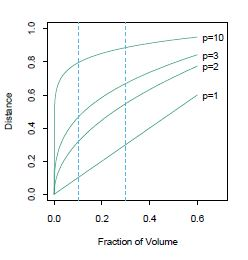
\includegraphics[width=0.9\textwidth]{cssofdimension}
\end{figure}

As seen in the picture, then with 10 features the side length has to be 80\% to cover 10\% of data.

For data fitted to a unit sphere the median distance from the center of
the sphere to the closest point is

\[
    d(p, n) = \left( 1- \left( \frac{1}{2}\right)^{1/n}\right)^{1/p}
\]

as seen in lecture \cite[p.~11]{lecture3}

But its not all bad. There are some blessings of dimensionality

\begin{itemize}
  \item Several features will be correlated and we can average over them
  \item Underlying distribution will be finite, informative data will lay on a low-dimensional manifold
  \item Underlying structure in data (samples from continuous processes, images etc) will give an approximate finite dimensionality.
\end{itemize}

\section{Dimension reduction}

How to decrease the dimension and identify the most important
variables, and get rid of the redundant or irrelevant variables.

\begin{itemize}
  \item Combinatoric search, forward and backward selection
  \item Regularization of parameters
  \item Projection to lower dimensions - latent variables
  \item Clustering of features
  \item Structuring parameter estimates
\end{itemize}

\subsection{Forward and backward selection}

If we do combinatoric search then: Try all possible combinations of features and select the optimal one.

The \textbf{Pros:} You will find the best combination., but the \textbf{Cons:} Number of combinations to test may be extremely large.

Forward-stepwise selection is a greedy algorithm, producing a nested sequence of models. In this sense it might seem sub-optimal compared to
best-subset selection. However, there are several reasons why it might be preferred:

\begin{itemize}
  \item Computational; for large p we cannot compute the best subset sequence, but we can always compute the forward stepwise sequence (even when $p \gg N$).
  \item Statistical; a price is paid in variance for selecting the best subset of each size; forward stepwise is a more constrained search, and will have lower variance, but perhaps more bias.
\end{itemize}

from \cite[p.~58]{friedman2016elements}

Backward-stepwise selection starts with the full model, and sequentially deletes the predictor that has the least impact on the fit. The candidate for dropping is the variable with the smallest Z-score. Backward selection can only be used when N > p, while forward stepwise can always be used.

\begin{figure}[H]
  \centering
  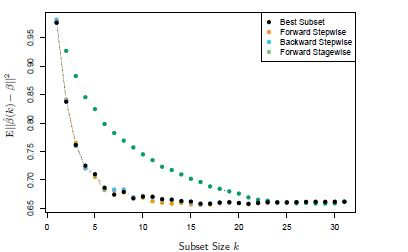
\includegraphics[width=0.9\textwidth]{forwardvsbackward}
\end{figure}

\section{Regularization}

Instead of controlling model complexity by setting a subset of
coefficients to zero we can shrink all the coefficients some way
towards zero.

Three established standard techniques

\begin{itemize}
  \item Ridge regression uses quadratic shrinkage, $L_2$-norm
  \item Lasso regression uses absolute-value shrinkage, $L_1$-norm
  \item Elastic net which is a hybrid method
\end{itemize}

\subsection{Ridge Regression}

Ridge regression shrinks the regression coefficients by imposing a penalty on their size. The ridge coefficients minimize a penalized residual sum of squares, it solves\cite[p.~61]{friedman2016elements}

\[
    \min\limits_\beta (Y - X \beta)^T (Y - X \beta) + \lambda \beta^T \beta
\]

Increased $\lambda$ will make the estimated $\beta$'s smaller but not exactly zero and We typically do not penalize the intercept $\beta_0$ \cite[p.~23]{lecture3}

Optimization of a weighted sum

\[
    \arg \min\limits_\beta || Y - X \beta ||^2_2 + \lambda ||\beta||^2_2
\]


\subsection{The Lasso}

The lasso is a shrinkage method like ridge, with subtle but important differences. \cite[p.~68]{friedman2016elements}

The Lasso regression solves

\[
    \min\limits_\beta (Y - X \beta)^T (Y - X \beta) + \lambda | \beta|
\]

Notice that the $L_2$-penalty is replaced by a $L_1$-penalty.\\

This makes the solution nonlinear in Y and a quadratic
programming algorithm is used to compute it.

For large enough $\lambda$ some of the $\beta$ will be set to exactly zero.

The effective numbers of parameters, equals the number of coefficients different from zero.

From lecture \cite[p.~27]{lecture3} then Lasso regularization will gear parameters towards zero.

\[
    \arg \min\limits_\beta || Y - X \beta ||^2_2 + \lambda ||\beta||_1
\]

The only difference from Ridge regression is that the regularization term is in absolute value. But this difference has a huge impact on the trade-off we’ve discussed before. Lasso method overcomes the disadvantage of Ridge regression by not only punishing high values of the coefficients $\beta$ but actually setting them to zero if they are not relevant. Therefore, you might end up with fewer features included in the model than you started with, which is a huge advantage

\subsection{Elastic net}

By combining the $L_1$ and the $L_2$-norm we obtain sparsity and shrinkage

\[
    \min\limits_\beta \frac{1}{2n} || Y - X \beta ||^2_2 + \lambda \left( \frac{1}{2} (1 - \alpha) ||\beta ||^2_2 + \alpha ||\beta||_2 \right)
\]

From lecture \cite[p.39]{lecture3} the Advantage: Combines the shrinkage of ridge and parameter selection of the lasso to obtain a robust sparse estimate.

The reasons to use elastic net is seen on lecture \cite[p.~49]{lecture3}

\begin{itemize}
  \item Get rid of irrelevant variables/select important variables (lasso)
  \item When p > n, the number of non-zero coefficients can exceed n unlike the lasso.
  \item Works well when covariates are highly correlated; allows us to “average” highly correlated features and obtain more robust estimates (grouping features).
\end{itemize}

The drawback is the issue of tuning two parameters. Use a grid search, a fine grid in $\lambda$ and fewer values for $\alpha$


\section{Multiple testing}

If we test one hypothesis at an $\alpha$-level of significance there is a chance $\alpha$ of falsely rejecting the hypothesis. \cite[p.52-53]{lecture3}

This is no longer the case if we do many tests!

The family-wise error rate (FWER) is the probability of at least one false rejection, and is a commonly used overall measure of error. \cite[p.~686]{friedman2016elements}

For M independent test at significance level $\alpha$

\[
    FWER = 1 - (1 - \alpha)^M
\]

\begin{itemize}
  \item 20 experiments conducted at a 5\% significance level
  \item Assume that the effect of different colors are independent, then $FWER = 1 - (1 - 0.05)^{20} \approx 0.64$
  \item There is 64\% probability of at least one false rejection
\end{itemize}

From lecture \cite[p.60]{lecture3} we should use the Bonferroni correction we rescale $\alpha$ with a number of tests.

So we reject a hypothesis if its $p$-value is below $\alpha/M$

From lecture \cite[p.~61]{lecture3} and \cite[p.~687]{friedman2016elements} we can look at the False Discovery Rate (FDR). We can have more significant findings if we allow for a few mistakes. The false discovery rate is a technique to control the number of
falsely detected significant features, where the FDR is

\[
    FDR = E \left( \frac{FP}{FP + TP}\right)
\]

where 

\begin{itemize}
  \item FP = False positives (false discoveries)
  \item TP = True positives (true discoveries)
\end{itemize}

If we accept hypotheses where $FDR < q$ then we will expect that
among our findings there will be $q$ mistakes.

\begin{itemize}
  \item Gain: We control false positives - added power.
  \item Cost: Increased number of false negatives.
\end{itemize}

We prefer to get a few false discoveries (percentage-wise) but gain more information, than ensuring no false discoveries and loosing some information.

Summary

\begin{itemize}
  \item Introduction
  \begin{itemize}
    \item The Curse of dimensionality
    \item The blessings of dimensionality
    \item Dimension reduction
  \end{itemize}
  \item Regularization
  \begin{itemize}
    \item Ridge, Lasso and Elastic Net
    \item Shrinkage and sparsity
    \item Best practices
  \end{itemize}
  \item Multiple hypothesis testing
  \begin{itemize}
    \item Why is it a problem
    \item Bonferroni correction
    \item False discover rate and Benjamini-Hochberg algorithm
  \end{itemize}
\end{itemize} 